\subsection{Lineare Funktionen}
Zu den einfachsten Funktionen gehören die linearen Funktionen. Alle linearen Funktionen (mit nur einer Variable) können in folgende Form gebracht werden: 
\begin{equation*}
f(x) = mx+t.
\end{equation*}
Hierbei ist $m$ der konstante Wert der Steigung:
\begin{equation*}
m= \frac{\triangle y}{\triangle x}=\frac{f(x_2)-f(x_1)}{x_2-x_1}
\end{equation*}
Die Konstante $t$ ist auch als $y$-Achsenabschnitt bekannt. Er wird so bezeichnet, da die Funktion für den $x$-Wert $0$ den Funktionswert $y = t$ annimmt. Viele komplizierte Funktionen werden am Ende doch wieder mit Hilfe einfacher lineare Funktionen angenähert. Lineare Funktionen lassen sich auf dem Computer leicht berechnen. Sie sind so prominent und verbreitet, dass es für sie eine eigene Vorlesung gibt: \textbf{Lineare Algebra}.


\begin{figure}[h!]
	\begin{center}
		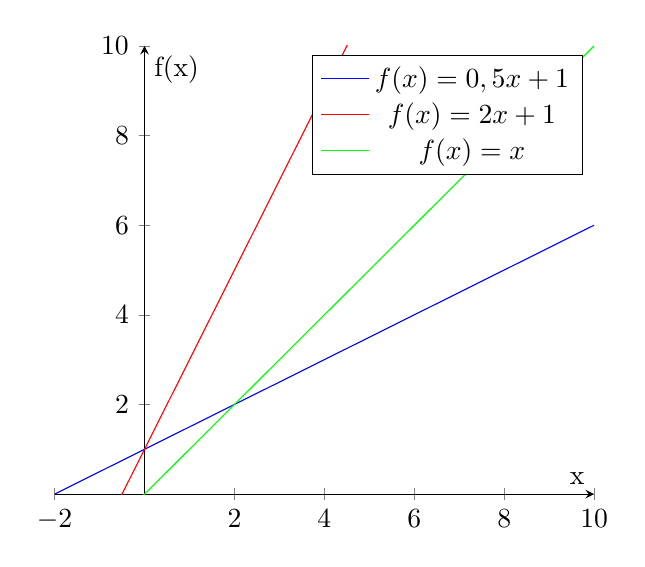
\begin{tikzpicture}[scale = 1.0]
		\begin{axis}[
		domain=-2:10,
		xmin=-2, xmax=10,
		ymin=-0, ymax=10,
		samples=400,
		axis y line=center,
		axis x line=middle,
		xlabel={x},
		ylabel={f(x)},
		]
		\addlegendentry{$f(x)=0,5x+1$}
		\addplot+[mark=none, color=blue] {0.5*x+1};
		\addlegendentry{$f(x)=2x+1$}
		\addplot+[mark=none, color=red] {2 * x+1};
		\addlegendentry{$f(x)=x$}
		\addplot+[mark=none, color=green] {x};
		\end{axis}
		\end{tikzpicture}
	\end{center}
	\caption{Beispiele linearer Funktionen in $\mathbb{R}\times\mathbb{R}$.}
	\label{fig:gerade}
\end{figure}
%Lineare Funktionen existieren in drei Ausprägungen. Geraden, Halbgeraden und Strecken. Eine Gerade ist unendlich lang, eine Strecke existiert nur zwischen zwei reellen Punkten und eine Halbgerade startet oder endet in genau einem Punkt. Der andere Teil geht ins Unendliche.

\subsubsection{Die Punktsteigungsform}
Um eine Gerade zu Definieren, sind immer zwei Dinge von Nöten:
\begin{itemize}
\item zwei Punkte $P_1 = (x_1, f(x_1)), P_2 = (x_2, f(x_2))$, welche auf der Geraden liegen \textbf{oder}
\item ein Punkt $P = (x_p, f(x_p))$ und die Steigung $m$ der Geraden
\end{itemize}
Im ersteren Fall berechnen wir $m$ nach obiger Gleichung $m = \frac{f(x_1) - f(x_2)}{x_1 - x_2}$ und sind im Fall 2. Um dann weiter zu verfahren, benötigt man die Punktsteigungsform, welche wie folgt lautet:
\begin{equation*}
f(x) = m \cdot (x-x_p) + y_p
\end{equation*}
$m$ ist hierbei wie gehabt die Steigung der Geraden und $x$ die Variable. $x_p$ und $f(x_p) = y_p$ sind jedoch die Koordinaten eines Punktes $P$, welcher auf der Geraden liegt. Nachdem man die Punktsteigungsform dann ausmultipliziert hat, besitzt man wieder die ganz normale Geradengleichung, wie oben beschrieben.

\subsubsection{Schnittpunkt zweier Geraden}
Ein Schnittpunkt zweier Funktionen ist ein Punkt, welcher sich auf beiden Graphen der Funktionen befindet. Wenn ein Punkt auf beiden Graphen sein soll, so muss er beide Funktionen erfüllen. Seien $f_1, f_2$ Geradenfunktionen so scheiden sich die von ihnen definierten Geraden im Punkt $S = (x, y)$ wenn
\begin{equation*}
f_1(x) = f_2(x) = y
\end{equation*}

\paragraph{Beispiel:}
Nehmen wir als Beispiel die Funktionen $f_1(x) = 4x$ und $f_2(x) = 12x - 23$. Es muss nun gelten 
\begin{equation*}
	f_1(x) = f_2(x) \iff 4x = 12x - 23 \iff -8x = -23 \iff x = \frac{23}{8}
\end{equation*}
Nun muss man den erhaltenen $x$-Wert nur noch in eine der beiden Gleichungen einsetzen und man erhält das Ergebnis oder wir schreiben frech
\begin{equation*}
S = \left( \frac{23}{8}, f_1(23/8) \right) = \left(\frac{23}{8}, \frac{23}{2} \right)
\end{equation*}
Der Schnittpunkt hat somit die Koordinaten $S = \left(\frac{23}{8}, \frac{23}{2} \right)$.

\subsubsection{Besondere Geraden}
\begin{itemize}
\item Besitzen zwei Geraden dieselbe Steigung, so sind diese parallel zueinander. Im Normalfall besitzen diese keinerlei Schnittpunkte. Eine besondere Art der Parallelität ist jedoch die Identität zweier Geraden. Identische Geraden besitzen unendlich viele Schnittpunkte.
\item Sind zwei Geraden senkrecht (im rechten Winkel) zueinander, so ist das Produkt ihrer Steigungen -1: $m_1 \cdot m_2 = -1$.
\item Eine  \textcolor{red}{Tangente} ist eine Gerade, die mindestens einen Punkt, sowie an diesem Punkt die Steigung mit einer Kurve gemeinsam hat. Man sagt auch, sie berührt den Punkt der Kurve an dieser stelle.
\item Eine  \textcolor{red}{Sekante} schneidet eine Kurve in zwei Punkten.
\end{itemize}